
\documentclass[11pt]{article}

\usepackage{amsmath} %import amsmath for align command
\usepackage{cite} %import package for using bibtex bibliography
\usepackage{graphicx} %import package for inserting figures from image files
\usepackage{mathtools} %import package for using certain symbols such as eq. arrows
\usepackage{tikz} %import package for creating figures
\usepackage{booktabs}
\usepackage{siunitx}
\usepackage[T1]{fontenc}
\usepackage[font=small,skip=0pt]{caption}


\usepackage{placeins}
\usepackage{array}
\newcolumntype{P}[1]{>{\centering\arraybackslash}p{#1}}

\usepackage[nodisplayskipstretch]{setspace}


\usepackage{titlesec}
\titlespacing{\section}{0pt}{0.8\baselineskip}{0.8\baselineskip}
\titlespacing{\subsection}{0pt}{0.675\baselineskip}{0.675\baselineskip}
\setlength{\abovecaptionskip}{2pt plus 2pt minus 5pt}

% for referencing links
\usepackage{hyperref}
\hypersetup{
	colorlinks=true,
	linkcolor=blue,
	filecolor=magenta,
	urlcolor=cyan,
}

% \usepackage{apacite}

\usepackage{algorithm}
\usepackage[noend]{algpseudocode}
\usepackage{textcomp}
\usepackage{subcaption}

%change default margins
\setlength{\topmargin}{-.75in}
\setlength{\textheight}{9.5in}

\setlength{\oddsidemargin}{0in}
\setlength{\evensidemargin}{0in}
\setlength{\textwidth}{6.6in}

\graphicspath{{aima/images/}}

\newcommand{\urlNewWindow}[1]{\href[pdfnewwindow=true]{#1}{\nolinkurl{#1}}}
\newcommand{\problemone}{grid world problem}
\newcommand{\Problemone}{grid world problem}
\newcommand{\problemtwo}{choice suggestion problem}
\newcommand{\Problemtwo}{choice suggestion problem}
\newcommand{\expnumber}[2]{{#1}\mathrm{e}{#2}}

\begin{document}

%create title
\title{Deep Reinforcement Learning Nanodegree\\
	   Project 1 -- Navigation Report}
\author{\vspace{-1mm}Chris Cadonic\\
chriscadonic@gmail.com}
\maketitle
\vspace{-1.5em}

\section{Introduction}

As part of the first project for the deep reinforcement learning nanodegree, I built and trained an agent that learns how to navigate through a world with yellow and blue bananas in an effort to maximize how many yellow bananas it can acquire.

\subsection{Environment Overview}

In the Unity-ML environment provided, the agent navigates through a world filled with yellow and blue bananas. As the agent moves through the world, if it comes into contact with a banana it will pick it up, receiving a reward of +1 if it picks up a yellow banana and -1 if it picks up a blue banana. Its goal is to maximize its reward for a single play session where it navigates and tries to pick up as many yellow bananas while avoiding blue bananas. The game is considered solved if it achieves an average score over 100 games of \textbf{+13}.

As the agent interacts, it receives information from the environment of the form:
\textbf{insert state info}

Interactions available to the agent include moving in one of four directions:
\begin{itemize}
	\item move forward,
	\item move backward,
	\item turn left,
	\item turn right,
\end{itemize}
with these four actions forming the action space $\mathcal{A}$. The agent solves the game by understanding what the optimal action is to take in each of the possible states that it finds itself in.

\section{Approach}

Initially I had approached this problem by first attempting to use Q-learning as
a first benchmark, but given the continuous nature of the state space
$\mathcal{S}$ this would also necessitate discretization or tile coding the
space. For this reason, I instead chose to implement a vanilla DQN (Deep
Q-network) and iteratively improve it to achieve better performance.

\subsection{DQN}

My first complete algorithm for DQN leveraged a simple multi-layer perceptron
using the following architecture:

\FloatBarrier

\begin{figure}[!ht]
    \centering
	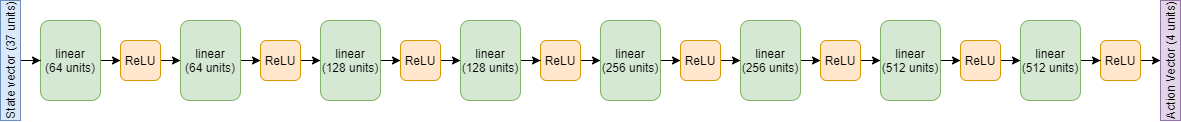
\includegraphics[width=\linewidth]{images/dqn-architecture.png}
    \caption{The 8-layer MLP used in the DQN algorithm.}
    \label{fig:dqn-architecture}
\end{figure}

\FloatBarrier

I chose to experiment with a deeper model that leveraged increasingly wider linear layers,
 ending up with an 8-layer neural network with units of sizes [64, 64, 128, 128, 
 256, 256, 512, 512] and $ReLU$ activation functions between each layer.

I also needed to experiment hyperparameter tuning for the following 
hyperparameters:

\FloatBarrier

\begin{table}[!ht]
	\centering
	\begin{tabular}{ c | c }
	\textbf{hyperparameter} & \textbf{values} \\
	\hline
	$\epsilon_{decay}$ & $[0.99, 0.996, 0.999, 0.9999, 0.99999]$ \\
	$\alpha$ & $[0.00005, 0.0001, 0.0005, 0.001, 0.005]$ \\
	$\tau$ & $[0.005, 0.01, 0.1]$ \\
	$\gamma$ & $[0.8, 0.9, 0.95, 0.99]$ \\
	\hline
	\end{tabular}
	\caption{Hyperparameters experimented with to train an agent using DQN.}
	\label{tbl:hyperparameters}
\end{table}

\FloatBarrier

Even though learning performance from the vanilla DQN was quite good (see results in
Fig. \ref{fig:dqn-performance}), I wanted to see explore options to determine if
performance could be improved.

\subsection{Improving DQN}

Since I had the least experience with implementing prioritized experience
replay, this was the first method I chose to expand on my vanilla DQN.

\subsubsection{Prioritized Experience Replay}

Using prioritized experience replay expands on the idea of sampling from the
replay buffer to provide experience tuples for the agent to learn from. In the
original DQN algorithm, this sampling is uniform across all stored experience
tuples in the replay buffer, whereas prioritized experience replay
\textit{prioritizes} experience tuples that resulted in a larger loss from
expected Q-values, capturing that these tuples may have been more impactful
during the learning process and will likely be more useful to sample more often
than lesser impactful experience tuples.

In order to expand on my initial implementation, I changed the following:
- storage of 


\subsubsection{Double DQN}


\subsubsection{Dueling DDQN}

\FloatBarrier

\begin{figure}[!ht]
    \centering
    \caption{}
    \label{fig:dueling-architecture}
\end{figure}

\FloatBarrier

\section{Results and Discussion}

\subsection{Learning Performance}

The results in Fig. \ref{fig:dqn-results} show that the the vanilla DQN
algorithm with the architecture shown in Fig. \ref{fig:dqn-architecture} achieved 
quite good performance, solving the navigation problem in 1185 episodes. That is, 
achieving an average score of +13 over 100 episodes after the 1185th episode.

\FloatBarrier

\begin{figure}[!ht]
	\centering
	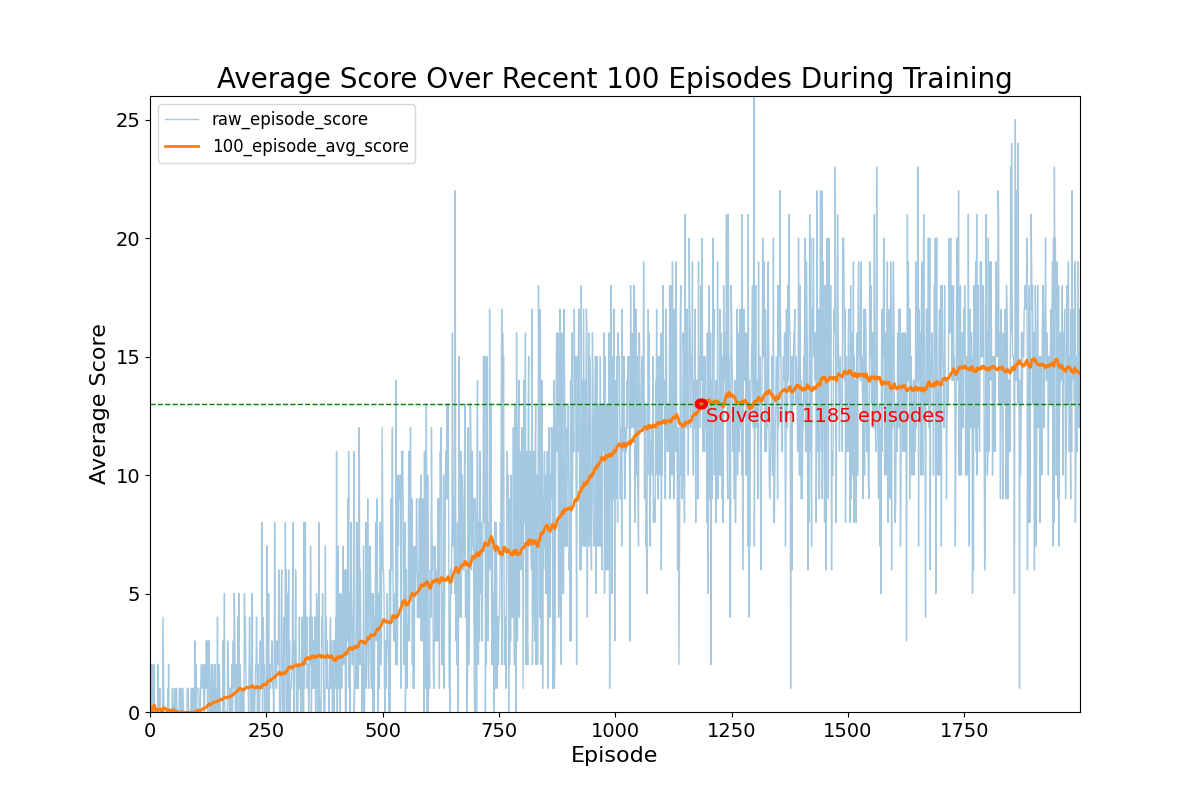
\includegraphics[width=0.8\linewidth]{images/dqn-results.png}
	\caption{}
	\label{fig:dqn-results}
\end{figure}

\FloatBarrier

After running experimentation over the parameters listed in Tbl. \ref{tbl:parameters} 
the optimal parameters were:
\begin{itemize}
	\item $\epsilon_{decay} = 0.996$,
	\item $\alpha = 0.001$,
	\item $\tau = 0.01$,
	\item $\gamma = 0.99$.
\end{itemize}

Evident in the learning performance of the agent, not only was the agent able to 
solve the navigation problem fairly quickly, but it was able to continue to improve 
beyond this, likely because I also enforced a minimum value on $\epsilon_{min} = 0.05$ 
to ensure that the agent is never \textit{entirely} acting greedily.

\subsection{Next Steps}



\section{Conclusion}




\bibliographystyle{unsrt}
\bibliography{sample}
% \begin{thebibliography}{9}
% \bibitem{littman}
% Leslie~Pack Kaelbling, Michael~L Littman, and Andrew~W Moore.
% \newblock Reinforcement learning: A survey.
% \newblock {\em Journal of artificial intelligence research}, 4:237--285, 1996.
% \end{thebibliography}

\end{document}
